\chapter{ARC sample of radio-galaxies}
\label{chp:dataset}
\captionsetup{width=0.75\textwidth}


The ALMA Radio-source Catalogue (ARC) Survey, is a full spectroscopic archival survey conducted in order to study the impact relativistic jet outflows have on the evolution of radiogalaxies.

\section{Data selection of ARC galaxies} \label{sec:ARCsurv}

The ARC survey is been led by Kalliopi Dasyra, has been presented and exhaustively described by Anelise Audibert, Kalliopi Dasyra, Michalis Papachristou, Juan Antonio Fernández Ontiveros, Ilaria Ruffa, Laura Bisigello, Françoise Combes, Philippe Salomé and Carlotta Gruppioni in their work of  Audibert et al. (2022)\cite{Audibert2022}.\\
The team of Audibert et al. (2022)\cite{Audibert2022} made use of the VizieR catalogue (operated at CDS, Strasbourg, France, DOI : \url{10.26093/cds/vizier}), the SIMBAD Database (operated at CDS, Strasbourg, France, DOI : \url{10.1051/aas:2000332}), the NASA/IPAC Extragalactic Database (operated at Caltech, Pasadena, California, USA, DOI: \url{10.1007/978-94-011-3250-3\_10 }) with the \code{astroquery}\cite{astroquery} access tool in the \code{python} programming language to collect the data. \\  
The survey consists of millimetre and sub-millimetre bright objects (mostly bright quasars) that can serve as flux, phase and band-pass calibrators for the  Atacama Large Millimetre/submillimetre Array (ALMA).\\
All sources have spectroscopically determined redshift with at least two detected CO transition lines. The sources selected fulfill the $1.4$GHz-to-$24$μm flux criterion to ensure that their radio emission is associated with Supermassive Black Hole (SMBH) accretion, and have a $1.4$GHz flux above $0.4$Jy. The resulting radiogalaxy sample consists of 120 sources and resembles the flux distribution of the NRAO VLA Sky Survey (NVSS) $1.4$GHz imaging survey.\\ 
In Figure \ref{fig:ARC_field}, the ARC sample of 120 radiogalaxies is shown with their redshift distribution. The effective field-of-view (FOV) of the ARC survey is $\Omega_{\mbox{\tiny{eff, ARC}}} = 75 \mbox{arcmin}^2 $.
%The effective field-of-view (FOV) for each galaxy of the ARC survey is $\Omega_{\mbox{\tiny{eff, ARC}}} = 75 \mbox{arcmin}^2 $, while (as it is shown in the right panel of Figure \ref{fig:ARC_field}) the total ARC coverage of the celestial sphere is north of $\mbox{dec}_{\mbox{\tiny{min}}}=-80^o= -4\pi/9 \;\mbox{radian}$ and south of $\mbox{dec}_{\mbox{\tiny{max}}}=80^o = 4\pi/9 \;\mbox{radian}$, leading to 
%\begin{equation}
%\Omega_{\mbox{\tiny{tot, ARC}}} = \int_{0}^{2\pi}\,d\phi\, \int_{-4\pi/9}^{4\pi/9}\, \cos \theta\,d\theta = 2\pi \times (2\sin\frac{4\pi}{9}) \; \mbox{steradian}= 3.94 \pi \; \mbox{steradian}
%\label{eq:OmegaTotARC}
%\end{equation}
\begin{figure}
    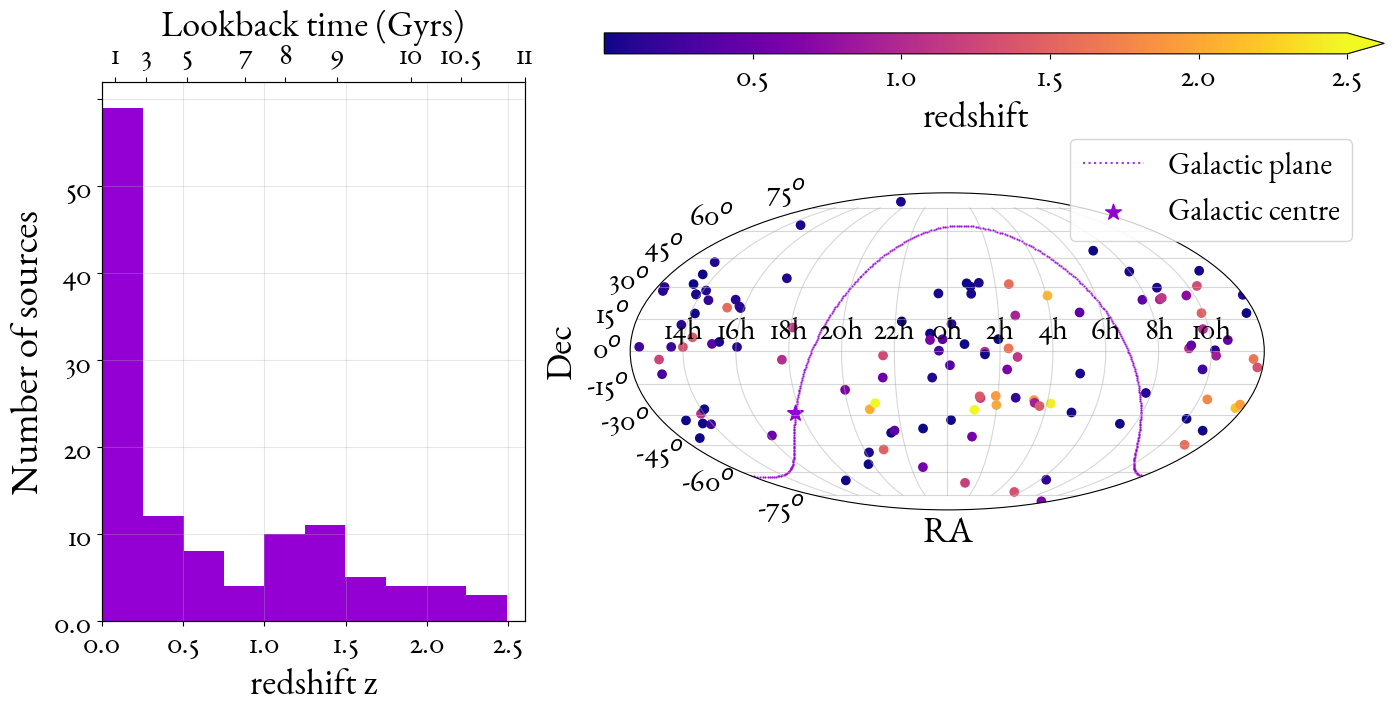
\includegraphics[width=\textwidth]{figures/DataSet/ARCfield_redshiftleft_T.png}
    \caption{The ARC survey. Left panel: histogram of the redshift spanning of the 120 ARC sources. Right panel: Projection of the ARC sample in the celestial sphere.}
    \label{fig:ARC_field}
\end{figure}
%---------------------------------------------------------%
%---------------------------------------------------------%
%---------------------------------------------------------%

\section{SED data acquisition \textit{\&} compilation}
%To construct the SEDs of our sources we use public %from georg CHANGE!
The aquisition of multiwavelength Spectral Energy Distribution (SED) data for each of the 120 ARC sources has been accomplished by Michalis Papachristou, with the use of the database services of the VizieR catalogue, the SIMBAD Database, the NASA/IPAC Extragalactic Database and the \code{astroquery}\cite{astroquery} access tool. The SEDs consist of all available photometric data from rest-frame far-ultraviolet (FUV) to radiofrequencies, as shown in Figure \ref{fig:RawSEDs}, denoted as "Full Data". 
%Full table \ref{app:Dataset}
%---------------------------------------------------------%
%---------------------------------------------------------%
%---------------------------------------------------------%

\section{Data cleaning}\label{sec:DataClean}
%Because of this, we included in our analysis all the available photometric data from ultraviolet (UV) and infrared (IR) full-sky coverage surveys when were available (Fig. 1). The chosen filters cover UV to mid-IR with up to 68 bands as detailed below.This selection was made to cover the rest-frame UV to near-IR fluxes up to z = 2.5 for all sources. This will allow a good estimate of the SED, especially on the host galaxy emission.%GEORGAKAKIS-CHANGE IT AS MUCH AS POSSIBLE
%-----------------------------------------------------%
%Elaborate
%The sample of galaxies \cite{Audibert2022}:  ALMA Radio Source Catalogue (ARC), ALMA calibrators,  with CO(1–0), CO(2–1), CO(3–2), or CO(4–3) emission spectral lines, representative of the NVSS radio galaxy survey NVSS 1.4 GHz
% For the compilation of data the following database services are used: NASA/IPAC Extragalactic Database (NED)\cite{NED} \footnote{\url{ned.ipac.caltech.edu}}, Simbad Astronomical Database \cite{Simbad} \footnote{\url{simbad.u-strasbg.fr/simbad}}, and VizieR Catalogue \cite{VizieR} \footnote{\url{vizier.cds.unistra.fr/viz-bin/VizieR}} 
The full multiwavelength SED data compiled include photometric observations from different telescopes with a variety of apertures taken through individual filter bands, as well as spectrograms, which offer a higher spectral resolution compared to photometry.\\
To ensure that each photometric data point corresponds to the integrated light of the full extend of the observed source, Athanasia Gkogkou (who worked on a small subset of these galaxies) imposed the criterion that the aperture of each photometric measurement must include the entire angular size (as described in equation \ref{eq:AngS}) of the galaxy observed in the given redshift, assuming a representative characteristic diametre $d_{\mbox{\tiny{gal}}}=30 $ kpc, excluding all observations with smaller aperture (since they would underestimate the flux) as well as all observations with much wider aperture (since integrated flux from nearby sources can contaminate and overestimate the flux). \\
Markos Polkas developed a routine in order to make a systematic selection of SED data points that are representative of each ARC galaxy's flux without assuming a $30$ kpc diametre and a routine in order to select the upper limit of the AGN's accretion disk emission, as shown in Figure \ref{fig:RawSEDs}, denoted as "Reduced Data" and "BBB upper limit".\\ \\
In the present work the end product of the compiled and cleaned SED data of ARC galaxies is used. Given the spectroscopic redshift information of every source (relevant details in Appendix \ref{app:Dataset}), each SED in this work is plotted and analysed in the source's rest frame, with the SED intensity being converted to units of luminosity [erg/s].

\begin{figure}
\centering
  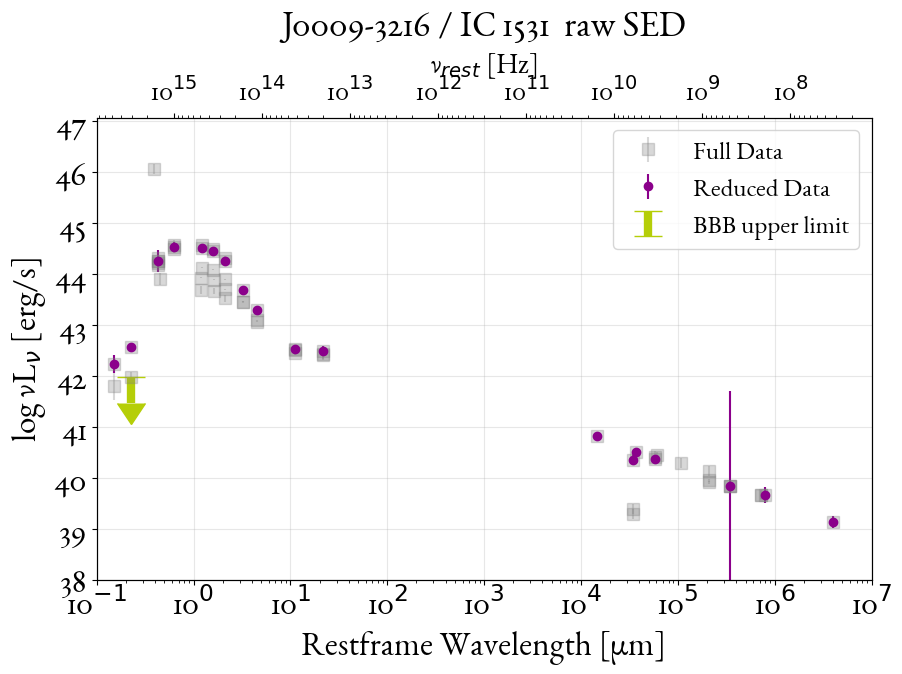
\includegraphics[width = 0.85\textwidth]{figures/DataSet/1_rawSED_16.png}
  %\qquad 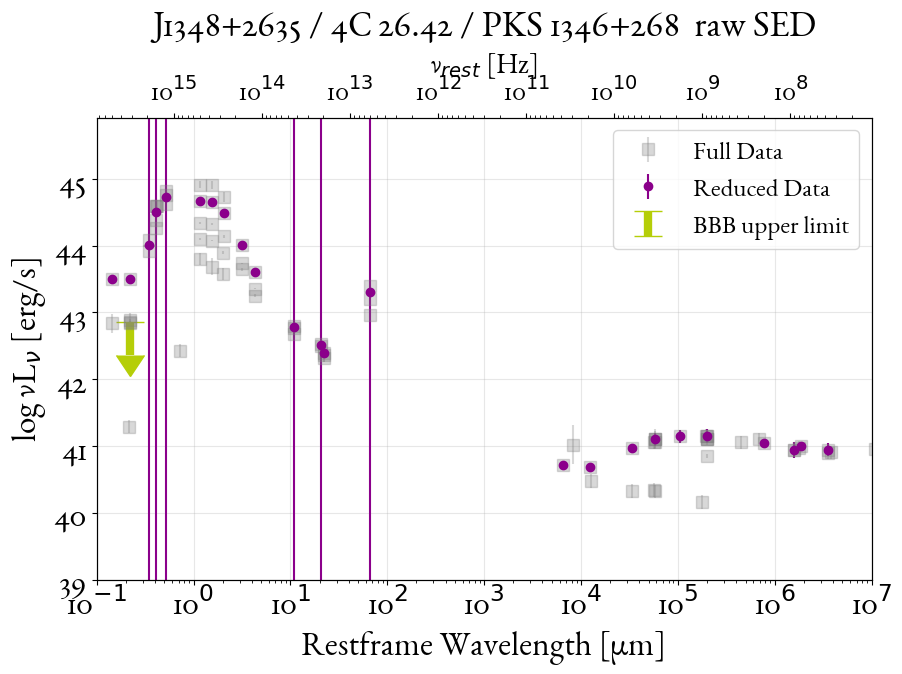
\includegraphics[width = 0.49\textwidth]{figures/DataSet/56_rawSED_4326.png}}\\
  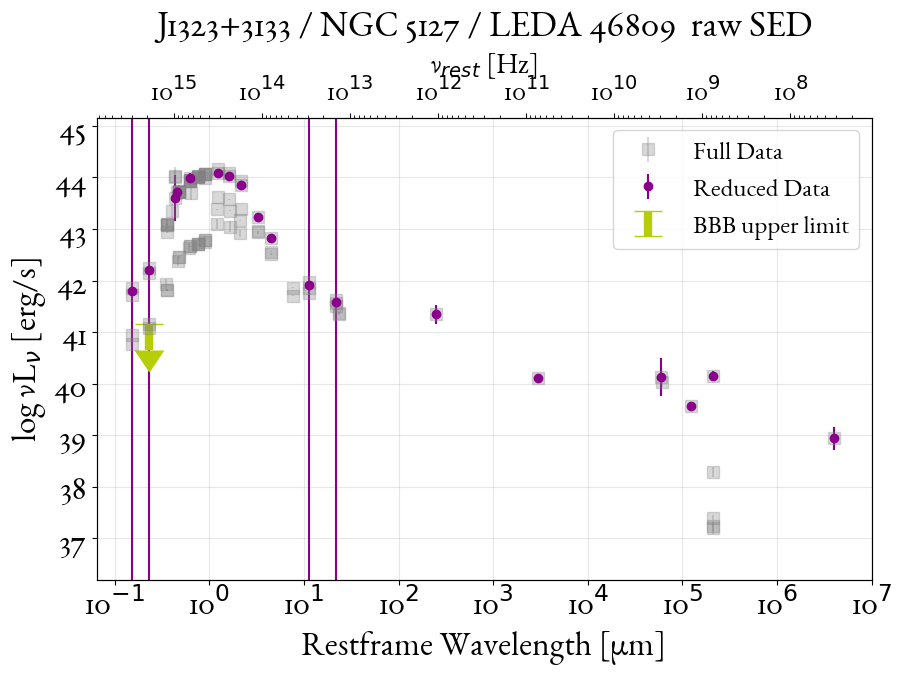
\includegraphics[width = 0.85\textwidth]{figures/DataSet/91_rawSED_5255.png}
  \caption{Raw SEDs of two ARC galaxies. Data integration by Michalis Papachristou, seen as the data points labeled "Full Data". Data reduction by Markos Polkas, the selection of the SED photometry (marked as "Reduced Data") and the upper limits for the accretion disk emission (marked as "BBB upper limit").}
  \label{fig:RawSEDs}
\end{figure}





%redshift values \href{}



